\chapter{Background}
\label{chap:background}

This chapter provides the foundational concepts necessary to understand the proposed methodology. We begin by reviewing the fundamental principles of neural networks and optimization via gradient descent. We then discuss the architectural scaling of foundation models, the transfer learning paradigm, and the resulting communication bottlenecks inherent in decentralized distributed systems. Next, we examine the core federated learning framework (including client drift under statistical heterogeneity, the Dirichlet partitioning methodology, and server-side adaptive optimization) before quantifying the communication costs that motivate parameter-efficient methods. We then survey the parameter-efficient fine-tuning landscape, focusing on Low-Rank Adaptation and the asymmetric properties of its factor matrices, and analyze the spatial aggregation inconsistency problem that arises when integrating low-rank adapters into federated training. Finally, we explore the geometric monitoring foundations and temporal optimization mechanisms underlying Federated Dynamic Averaging, establishing the theoretical mechanics that underpin FDA-RoLoRA presented in Chapter~\ref{chap:methodology}.

\section{Neural Networks and Optimization}
\label{sec:nn_sgd}

\subsection{Neural Networks}
Supervised learning with neural networks is a cornerstone of modern machine learning, enabling systems to learn complex mappings from input data to desired outputs. In this setting, the objective is to learn a function parameterized by a neural network that generalizes well to unseen data.

In the forward pass, an input vector $x$ is processed through the network layers to produce a prediction. This can be formally denoted as:
\begin{equation}
    \hat{y} = f_w(x)
    \label{eq:forward_pass}
\end{equation}
where $f_w$ represents the neural network parameterized by a set of weights $w$. The goal of the learning process is to adjust $w$ such that the predictions $\hat{y}$ closely match the true labels $y$.

To quantify the performance of the network, we define a loss function. For a dataset containing $n$ samples, the empirical risk or average loss $\mathcal{L}(w)$ is computed as:
\begin{equation}
    \mathcal{L}(w) = \frac{1}{n} \sum_{i=1}^{n} \ell(f_w(x_i), y_i)
    \label{eq:empirical_loss}
\end{equation}
where $\ell(\cdot, \cdot)$ is a sample-wise loss function (e.g., cross-entropy for classification). Minimizing this loss function with respect to the parameters $w$ is the central optimization problem in training neural networks.

\subsection{Gradient Descent}
The minimization of the empirical risk is typically performed using gradient-based optimization. The gradients of the loss function with respect to the network weights, denoted as $\nabla_w \mathcal{L}(w)$, are computed efficiently using the backpropagation algorithm. Backpropagation systematically applies the chain rule of calculus from the output layer back to the input layer, distributing the error gradients across all intermediate parameters.

With the gradients computed, the network weights are iteratively updated using Gradient Descent (GD). The fundamental GD update rule at training step $t$ is defined as:
\begin{equation}
    w_{t+1} = w_t - \eta \nabla_w \mathcal{L}(w_t) = w_t - \eta \frac{1}{n} \sum_{i=1}^{n} \nabla_w \ell(f_{w_t}(x_i), y_i)
    \label{eq:gd_update}
\end{equation}
where $\eta$ is the learning rate, a hyperparameter controlling the step size of the update. In standard GD, the true gradient is computed over the entire dataset of size $n$ at each iteration.

\subsection{Stochastic Gradient Descent}
In practice, computing the full gradient over the entire dataset is computationally prohibitive for large datasets. Therefore, Stochastic Gradient Descent (SGD) and its mini-batch variant are universally employed. In mini-batch SGD, the true gradient is approximated using a small subset or mini-batch of $m$ samples (where $m \ll n$). The update rule becomes:
\begin{equation}
    w_{t+1} = w_t - \eta \frac{1}{m} \sum_{j=1}^{m} \nabla_w \ell(f_{w_t}(x_{i_j}), y_{i_j})
    \label{eq:sgd_update}
\end{equation}
This introduces stochasticity into the optimization process, which not only accelerates each training iteration by reducing the computational cost per step, but can also aid the model in escaping shallow local minima. 

While vanilla SGD is effective, modern deep learning often utilizes adaptive optimization algorithms, such as Adam. These optimizers maintain moving averages of past gradients and squared gradients to scale the learning rate on a per-parameter basis, accelerating convergence and improving stability. As we will discuss in later sections, the concepts behind adaptive optimizers are highly relevant when addressing the challenges of server-side optimization in distributed settings.

\section{Foundation Models and the Transformer Architecture}
\label{sec:foundation_models}

In recent years, the machine learning paradigm has undergone a profound shift, transitioning from task-specific neural networks to large-scale pre-trained \emph{foundation models} \cite{bommasani2021opportunities}. Foundation models, which include Large Language Models (LLMs) such as GPT-3 \cite{brown2020language}, RoBERTa \cite{liu2019roberta}, and Llama \cite{touvron2023llama}, are trained on vast unlabeled datasets using self-supervised learning, enabling them to be adapted to a broad range of downstream tasks with minimal structural modifications.

At the core of virtually all modern foundation models is the Transformer architecture introduced by Vaswani et al. \cite{vaswani2017attention}. Unlike traditional Recurrent Neural Networks (RNNs) or Convolutional Neural Networks (CNNs) that process sequential data step-by-step or through localized receptive fields, the Transformer relies fundamentally on the multi-head self-attention mechanism. For an input representation matrix $X \in \mathbb{R}^{n \times d}$, self-attention projects $X$ into Query ($Q$), Key ($K$), and Value ($V$) representations using parameter matrices $W_Q, W_K, W_V \in \mathbb{R}^{d \times d_k}$:
\begin{equation}
    \text{Attention}(Q, K, V) = \text{softmax}\left( \frac{Q K^\top}{\sqrt{d_k}} \right) V
    \label{eq:self_attention}
\end{equation}
This formulation allows the network to capture pairwise interactions between all tokens in a sequence simultaneously, enabling high computational parallelization during training.

However, the empirical success of foundation models has been driven by massive parameter scaling. Modern architectures frequently range from hundreds of millions (e.g., RoBERTa-Large with 355M parameters) to tens or hundreds of billions of trainable parameters (e.g., Llama-2 with 7B to 70B parameters) \cite{touvron2023llama}. This unprecedented scale introduces severe computational and memory challenges. Full fine-tuning (updating all weights $w \in \mathbb{R}^d$ during downstream optimization) requires storing activation states, gradients, and optimizer momentum buffers for billions of parameters simultaneously. Consequently, deploying and adapting foundation models shifts machine learning from single-device training to distributed infrastructures and parameter-efficient adaptation paradigms.

The practical utility of foundation models is realized through the \emph{transfer learning} paradigm. During the first phase, a model is pre-trained on a massive, general-purpose corpus using self-supervised objectives (e.g., masked language modeling for encoder models or next-token prediction for autoregressive models), learning broad linguistic and semantic representations. In the second phase, this pre-trained model is \emph{fine-tuned} on a smaller, task-specific labeled dataset (such as sentiment classification, natural language inference, or instruction following \cite{ouyang2022training}) by continuing gradient-based optimization on the downstream objective. The key insight is that the representations learned during pre-training transfer effectively to downstream tasks, enabling strong performance with far less task-specific data than training from scratch. However, standard fine-tuning still requires updating all $d$ parameters, which motivates the parameter-efficient approaches discussed in subsequent sections.

\section{Distributed Machine Learning}
\label{sec:distributed_ml}
As the complexity of tasks and the volume of available data have grown, both datasets and neural network architectures have become too large to be efficiently processed on a single machine. This computational bottleneck has motivated the development of distributed machine learning systems, where the training process is partitioned across multiple worker nodes or machines. A comprehensive landscape of modern parallel and distributed learning methodologies, including detailed taxonomies of synchronization models and parallelism paradigms, is surveyed by Subasi et al. \cite{subasi2023landscape}.

Distributed training strategies generally fall into two categories: data parallelism and model parallelism \cite{subasi2023landscape}. In data parallelism, the dataset is divided into partitions distributed across the workers, while each worker maintains a complete replica of the model parameters. Conversely, in model parallelism, a single model is too large to fit in the memory of a single machine, so its layers or components are distributed across multiple workers, while they all process the same data stream. Data parallelism is the most prevalent approach in scenarios scaling across large numbers of nodes.

In a standard data-parallel setup using synchronous SGD, all worker nodes independently compute gradients on their local data batches. Once all workers finish computing their local gradients, they synchronize by aggregating them, typically using an all-reduce operation. The globally averaged gradient is then used to update the model parameters across all nodes simultaneously. While mathematically equivalent to centralized mini-batch SGD with a larger batch size, synchronous SGD suffers from the straggler effect: the entire system must wait for the slowest worker to complete its computation before proceeding to the next step.

To mitigate the straggler problem, asynchronous SGD was introduced, often implemented via a parameter server architecture. In this paradigm, workers independently fetch the latest model parameters from a central server, compute gradients on their local data, and push the gradients back to the server without waiting for other workers. The server updates the model immediately upon receiving a gradient. However, this lack of synchronization introduces the staleness problem: a worker might compute gradients based on an older version of the model, and by the time it pushes its update, the server's model has already been updated by other workers. These stale gradients can introduce noise, destabilize training, and degrade final model performance.


The evolution of these distributed optimization techniques laid the groundwork for scaling machine learning. However, traditional distributed systems assume reliable communication networks, homogeneous compute nodes, and centrally accessible data. The emergence of privacy concerns and the proliferation of edge devices necessitated a paradigm shift, giving rise to Federated Learning as a privacy-preserving variant of distributed learning that addresses the unique challenges of decentralized data.

\section{Federated Learning and Communication Bottlenecks}

Federated Learning significantly diverges from classical distributed learning by focusing on privacy preservation across decentralized edge devices. Unlike traditional distributed setups with centrally managed data and homogeneous reliable workers, FL must navigate highly heterogeneous local datasets, unreliable network connections, and computationally constrained clients.

\subsection{Federated Averaging}
Federated Learning \cite{kairouz2021advances} enables collaborative machine learning across a set of decentralized clients $K$ without centralizing private data. Figure \ref{fig:fl_overview} illustrates the typical FL lifecycle, comprising local training and global aggregation. Each client $k \in K$ retains its private dataset $\mathcal{D}_k$. The collective objective is to solve the distributed optimization problem:
\begin{equation}
    \min_{w \in \mathbb{R}^d} F(w) = \frac{1}{|K|} \sum_{k \in K} F_k(w)
    \label{eq:fl_objective}
\end{equation}
where $F_k(w) = \mathbb{E}_{x \sim \mathcal{D}_k} [\ell(w; x)]$ represents the local objective function of client $k$ over a loss function $\ell(w; x)$ parameterized by the model weights $w \in \mathbb{R}^d$.

\begin{figure}[htbp]
    \centering
    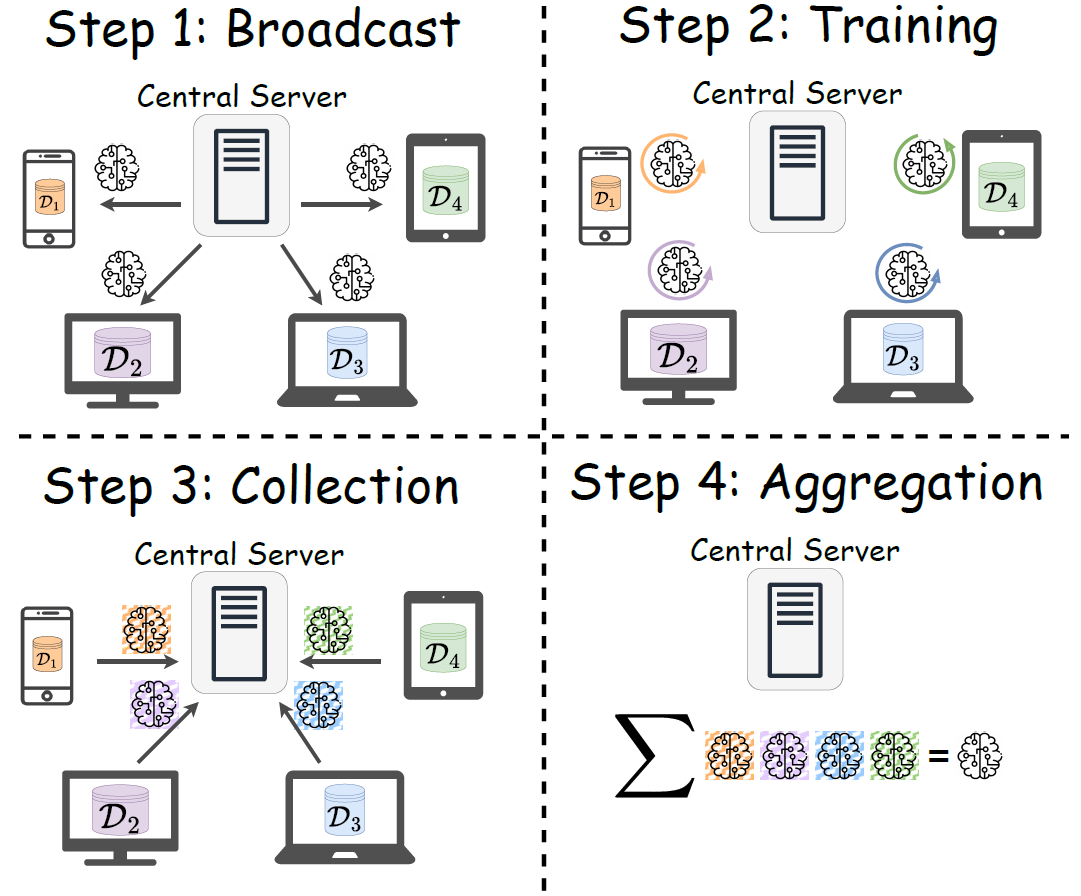
\includegraphics[width=0.60\textwidth]{figures/federated averaging.png}
    \caption{Chronological sequence of a Federated Learning communication round (broadcast, local client training, update collection, and server aggregation). Figure reproduced from Theologitis et al. \cite{theologitis2025fda}.}
    \label{fig:fl_overview}
\end{figure}

To solve this problem, the standard Federated Averaging (FedAvg) algorithm \cite{mcmahan2017communication} operates in communication rounds. At round $t$, the server selects a client cohort $S_t \subset K$ and broadcasts the global model $w_t$. The selected clients initialize their local models as $w_{t,0}^{(k)} = w_t$ and perform $\tau$ local steps of Stochastic Gradient Descent (SGD):
\begin{equation}
    w_{t, j+1}^{(k)} = w_{t,j}^{(k)} - \eta \nabla \ell(w_{t,j}^{(k)}; x)
    \label{eq:fedavg_sgd}
\end{equation}
After training, clients transmit their local updates $\Delta_{t}^{(k)} = w_{t,\tau}^{(k)} - w_t$ to the server, which aggregates them to compute the next global model:
\begin{equation}
    w_{t+1} = w_t + \frac{1}{|S_t|} \sum_{k \in S_t} \Delta_{t}^{(k)}
    \label{eq:fedavg_agg}
\end{equation}

\subsection{FedOpt: Server-Side Adaptive Optimization}
For modern large foundation models, transmitting full weight vectors $w \in \mathbb{R}^d$ introduces severe spatial communication overhead. Furthermore, client-level statistics are often noisy, and clients are typically stateless, preventing the direct use of adaptive optimizers on edge devices. To address this, the FedOpt framework \cite{reddi2021adaptive} shifts adaptive optimization to the server. Leveraging the adaptive optimization principles (e.g., Adam) discussed in Section \ref{sec:nn_sgd}, FedOpt allows the server to aggregate client parameter displacements $\Delta_t^{(k)} = w_{t,\tau}^{(k)} - w_t$ across the cohort $S_t$:
\begin{equation}
    \Delta_t = \frac{1}{|S_t|} \sum_{k \in S_t} \Delta_{t}^{(k)}
    \label{eq:fedopt_displacement}
\end{equation}
Because local updates move along descent trajectories, $\Delta_t$ represents the average parameter displacement. In gradient-based server optimizers (e.g., FedAdam, FedAdamW), this quantity defines an effective server pseudo-gradient with an inverted sign:
\begin{equation}
    \nabla_{\text{pseudo}, t} = - \Delta_t = - \frac{1}{|S_t|} \sum_{k \in S_t} \Delta_{t}^{(k)}
    \label{eq:fedopt_pseudo}
\end{equation}
ensuring that standard gradient-descent update steps ($w_{t+1} = w_t - \eta_s \nabla_{\text{pseudo}, t}$, as formalized in Chapter~\ref{chap:methodology}) step in the direction of cumulative local progress, or equivalently through an additive displacement step:
\begin{equation}
    w_{t+1} = \text{ServerOpt}(w_t, \Delta_t)
    \label{eq:fedopt_update}
\end{equation}

The motivation for server-side adaptive optimization in federated learning is distinct from its role in centralized training. In centralized settings, adaptive optimizers like Adam \cite{kingma2015adam} accelerate convergence by maintaining per-parameter learning rate scaling. In federated settings, the pseudo-gradient $\nabla_{\text{pseudo}, t}$ suffers from compounded noise: it is computed from a sampled client subset $S_t \subset K$ rather than all clients, and each client's local update reflects multiple SGD steps on heterogeneous data rather than a single gradient evaluation. Server-side momentum buffers smooth these noisy pseudo-gradients across rounds, providing a more stable optimization trajectory.

Furthermore, federated clients are inherently \emph{stateless}: they do not persist optimizer state (momentum, variance estimates) between communication rounds, as each round begins with a fresh initialization from the global model. This precludes the use of adaptive optimizers at the client level across rounds, making the server the only entity capable of maintaining long-term optimization history. Additionally, in parameter-efficient adaptation regimes (detailed in Section~\ref{sec:peft}), decoupled weight decay (AdamW \cite{loshchilov2019decoupled}) at the server provides implicit regularization on adapter parameters, helping prevent overfitting to the heterogeneous local distributions encountered during federated training.

While FedOpt stabilizes training and accelerates convergence, it still relies on rigid, static synchronization schedules (fixed $\tau$), ignoring local optimization dynamics and leading to temporal communication inefficiencies.

\subsection{Client Drift and Statistical Heterogeneity}
\label{sec:client_drift}
A defining challenge in federated learning is the statistical heterogeneity of client data distributions. In practice, client datasets $\mathcal{D}_k$ are rarely independent and identically distributed (IID). Instead, they exhibit various forms of heterogeneity: \emph{label skew}, where different clients possess data from different subsets of classes; \emph{quantity skew}, where the number of local training samples varies significantly across clients; and \emph{feature skew}, where the underlying input distributions differ even for the same label \cite{zhu2021federated}.

Under non-IID data, the local objective functions $F_k(w)$ may have significantly different minimizers. When clients perform multiple steps of local SGD on their heterogeneous data, their parameters drift toward distinct local optima that diverge from the global optimum. This phenomenon, known as \emph{client drift} \cite{karimireddy2020scaffold}, causes the aggregated global update to deviate from the true gradient direction, degrading convergence speed and final model quality.

The severity of client drift is formally analyzed by Li et al. \cite{li2020convergence}, who establish convergence bounds for FedAvg under non-IID data that depend on the degree of gradient dissimilarity across clients. Various drift-mitigation strategies have been proposed: FedProx \cite{li2020federated} adds a proximal regularization term to constrain local updates to remain close to the global model, while SCAFFOLD \cite{karimireddy2020scaffold} introduces variance reduction through control variates that correct for client drift at each local step. These methods highlight that \emph{monitoring and controlling the divergence between local and global model states is fundamental to stable federated optimization}, a principle that directly motivates the variance-driven synchronization approach explored later in this chapter.

\subsection{Dirichlet-Based Data Partitioning}
\label{sec:dirichlet}
To rigorously evaluate federated algorithms under controlled non-IID conditions, the research community has adopted the Dirichlet distribution as the standard tool for synthetic data partitioning \cite{hsu2019measuring, yurochkin2019bayesian, zhu2021federated}. For a classification task with $C$ classes and $K$ clients, each client $k$ receives a class proportion vector $p_k \sim \text{Dir}(\alpha)$, where $\text{Dir}(\alpha)$ denotes the symmetric Dirichlet distribution with concentration parameter $\alpha > 0$. Training samples of each class are then allocated to clients according to these sampled proportions.

The concentration parameter $\alpha$ provides a single scalar knob to control the degree of heterogeneity. As $\alpha \to 0$, the sampled proportion vectors become increasingly peaked, producing extreme label skew where individual clients may hold data from only a single class. Conversely, as $\alpha \to \infty$, the proportions converge to a uniform distribution, recovering the IID setting. Intermediate values (e.g., $\alpha = 0.5$ or $\alpha = 1.0$) produce moderate heterogeneity that reflects realistic scenarios where clients have partial but imbalanced class coverage. This configurability makes the Dirichlet partitioning scheme essential for conducting systematic ablation studies across varying degrees of statistical adversity.

\subsection{Communication Cost Quantification}
\label{sec:comm_cost}
To make the communication bottleneck concrete, consider the per-round transmission cost for foundation models. For a transformer backbone such as \texttt{roberta-base} ($125\,\text{M}$ parameters), transmitting the full model weights in standard 32-bit floating point precision requires approximately $500\,\text{MB}$ per client per synchronization round (or $\sim 250\,\text{MB}$ in 16-bit half-precision). Across a modest cohort of 10 clients over a 100-round federated training run, this results in up to $500\,\text{GB}$ of raw model transfers over uplink-constrained edge networks. In multi-billion parameter foundation architectures (such as Llama-2-7B with $\approx 7\times 10^9$ parameters), a single full-model synchronization demands approximately $28\,\text{GB}$ in FP32 per client per round, which is completely intractable in distributed federated settings.

To overcome this prohibitive uplink requirement, parameter-efficient fine-tuning (PEFT) methods restrict trainable parameters to compact modular adapters. In particular, Low-Rank Adaptation (LoRA, formalised in Section~\ref{sec:peft}) decomposes weight updates into low-rank factor matrices. When targeting the attention projection matrices of \texttt{roberta-base} with a compact adapter rank $r = 4$ (typically $r \in \{4, 8\}$), the communicated payload drops from $500\,\text{MB}$ to under $1\,\text{MB}$ per client per round, achieving a spatial compression ratio exceeding $500\times$. This substantial reduction demonstrates why low-rank parametrization is essential to make federated training of foundation models feasible across bandwidth-constrained edge networks.

\section{Parameter-Efficient Fine-Tuning}
\label{sec:peft}
The massive scale of foundation models renders traditional full fine-tuning (updating all $d$ parameters for a downstream task) increasingly impractical. Full fine-tuning requires storing not only the model weights but also the corresponding activation states, gradient tensors, and optimizer momentum buffers (e.g., first and second moment estimates for Adam) for every trainable parameter. For a model with $d$ parameters in mixed-precision training, the aggregate memory footprint can exceed $16d$ bytes, placing models with hundreds of millions or billions of parameters well beyond the capacity of commodity client hardware. Parameter-Efficient Fine-Tuning (PEFT) addresses this challenge by updating only a small subset of parameters while keeping the vast majority of pre-trained weights frozen.

\subsection{The PEFT Landscape}
\label{sec:peft_landscape}
Several families of PEFT techniques have been developed to balance parameter efficiency with representational capacity:
\begin{itemize}
    \item \textbf{Adapter Layers}: Introduced by Houlsby et al. \cite{houlsby2019parameter}, adapter modules inject small, learnable bottleneck layers between existing transformer feed-forward and self-attention projections. While parameter-efficient, they introduce structural changes that incur non-negligible inference latency.
    \item \textbf{Prefix Tuning}: Proposed by Li and Liang \cite{li2021prefix}, prefix tuning prepends learnable, continuous task-specific vectors directly to the key and value sequences of transformer attention layers, steering model behavior without modifying original parameters. However, prepending prefixes reduces the effective sequence length available for downstream context.
    \item \textbf{Prompt Tuning}: A further simplification of prefix tuning that prepends virtual token embeddings strictly to the input layer, offering high parameter economy but often exhibiting slower optimization convergence on complex tasks.
\end{itemize}

\subsection{Low-Rank Adaptation (LoRA)}
\label{sec:lora}
Among parameter-efficient adaptation paradigms, Low-Rank Adaptation (LoRA) \cite{hu2022lora} has emerged as the prevailing standard for both centralized and distributed environments. LoRA operates on the foundational hypothesis that weight updates during downstream task adaptation occupy a low intrinsic rank \cite{aghajanyan2021intrinsic}.

Rather than modifying a dense pre-trained weight matrix $W_0 \in \mathbb{R}^{d_{\text{out}} \times d_{\text{in}}}$ directly, LoRA parameterizes the weight update $\Delta W$ through a low-rank matrix decomposition:
\begin{equation}
    \Delta W = \frac{\alpha}{r} B A
    \label{eq:lora_factorization}
\end{equation}
where $A \in \mathbb{R}^{r \times d_{\text{in}}}$ denotes the down-projection matrix, $B \in \mathbb{R}^{d_{\text{out}} \times r}$ denotes the up-projection matrix, rank $r \ll \min(d_{\text{in}}, d_{\text{out}})$, and $\alpha$ is a constant scaling hyperparameter. The forward pass of a modified layer computes:
\begin{equation}
    h = W_0 x + \Delta W x = W_0 x + \frac{\alpha}{r} B A x
    \label{eq:lora_forward}
\end{equation}
Throughout fine-tuning, the pre-trained backbone weights $W_0$ remain completely frozen, receiving zero gradient updates. Only the compact factor matrices $A$ and $B$ are optimized. Under the canonical initialization scheme, $A$ is initialized with random Gaussian values $\mathcal{N}(0, \sigma^2)$, while $B$ is initialized to zero, ensuring that $\Delta W = \frac{\alpha}{r} B A = 0$ at training onset and the model's pre-trained predictions are exactly preserved prior to adaptation. The scaling factor $\frac{\alpha}{r}$ stabilizes the optimization dynamics when varying the adapter rank $r$, typically set such that $\alpha = 2r$. Figure~\ref{fig:lora_schematic} illustrates this architecture.

\begin{figure}[htbp]
    \centering
    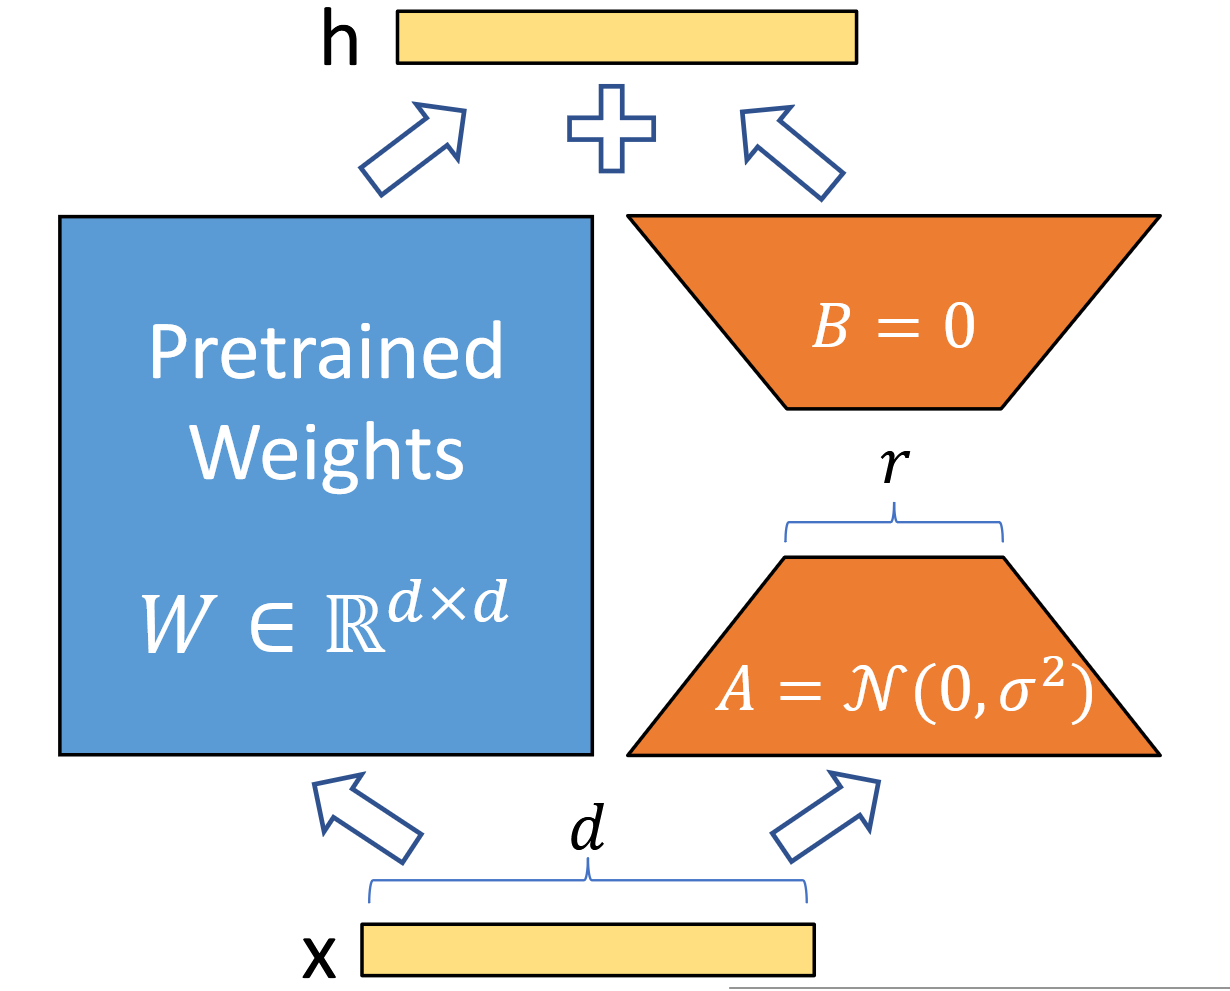
\includegraphics[width=0.4\textwidth]{figures/lora_figure.png}
    \caption{Low-Rank Adaptation (LoRA) schematic: decomposition of weight updates into low-rank matrices $A$ and $B$ alongside frozen pretrained weights $W$. Figure reproduced from Hu et al. \cite{hu2022lora}.}
    \label{fig:lora_schematic}
\end{figure} 

Unlike adapter layers, LoRA introduces zero additional inference latency: upon completion of training, the factorized update $\frac{\alpha}{r} BA$ can be folded directly into the pre-trained weights ($W_{\text{final}} = W_0 + \frac{\alpha}{r} BA$) via simple matrix addition. In centralized settings, extensions such as QLoRA \cite{dettmers2023qlora} (which integrates 4-bit NormalFloat base quantization) and AdaLoRA \cite{zhang2023adalora} (which dynamically allocates rank budgets across layers) have further highlighted the versatility of the low-rank paradigm.

\subsection{Structural and Dynamic Asymmetry in LoRA Matrices}
\label{sec:lora_asymmetry}
An essential, frequently overlooked property of the LoRA decomposition is the inherent asymmetry between its two factor matrices. Functionally, the down-projection matrix $A \in \mathbb{R}^{r \times d_{\text{in}}}$ compresses input features from high-dimensional representations into the low-rank bottleneck, whereas the up-projection matrix $B \in \mathbb{R}^{d_{\text{out}} \times r}$ expands compressed representations back to the original dimensionality. These distinct projection roles produce asymmetric gradient dynamics during backpropagation.

Furthermore, the canonical initialization scheme creates an acute temporal asymmetry: because $B = 0$ at initialization, the initial gradients with respect to $A$ ($\nabla_A \mathcal{L} \propto B^\top \nabla_h \mathcal{L}$) are initially zero, whereas the gradients with respect to $B$ ($\nabla_B \mathcal{L} \propto \nabla_h \mathcal{L} (A x)^\top$) immediately receive non-zero projections from the Gaussian-initialized $A$. Consequently, the optimization trajectories, convergence velocities, and parameter variance profiles of $A$ and $B$ diverge substantially during early training rounds, with matrix $B$ typically manifesting significantly higher drift. In federated learning, this asymmetry implies that treating both coordinate matrices identically during aggregation or synchronization scheduling is fundamentally suboptimal.

\section{Federated Low-Rank Adaptation}
\label{sec:fedlora}
Having established standard LoRA and the core FL framework, combining the two paradigms, formalized as Federated Low-Rank Adaptation (FedLoRA) \cite{yang2025federated}, is a natural evolution to reduce the massive communication costs of federated learning. In a typical FL setting, transmitting full model updates $w \in \mathbb{R}^d$ imposes severe network strain. By adopting LoRA, clients only train and transmit the low-rank matrices $A$ and $B$, which drastically reduces the spatial communication overhead of federated synchronization.

A comprehensive survey of FedLoRA \cite{yang2025federated} categorizes the primary challenges in this domain into distributed learning stability, data heterogeneity, and efficiency. To address these challenges, several frameworks have been proposed. For instance, FedIT \cite{zhang2023towards} applies standard federated averaging directly to LoRA parameters. To mitigate communication costs further and ensure exact updates, FFA-LoRA \cite{sun2024improving} freezes the down-projection matrices $A$ across all clients, allowing clients to update and transmit only the up-projection matrices $B$. Other approaches, such as FLoRA \cite{wang2024flora}, support heterogeneous-rank adapters among clients to accommodate varying device capacities.

Despite its benefits, aggregating independent low-rank matrices from clients introduces a critical issue known as \emph{LoRA Aggregation Discordance} \cite{yang2025federated}. When standard federated averaging (FedAvg) is applied separately to the client-specific matrices $A_i$ and $B_i$, it introduces a fundamental mathematical inconsistency:
\begin{equation}
    \frac{1}{N} \sum_{i=1}^{N} (B_i A_i) \neq \left( \frac{1}{N} \sum_{i=1}^{N} B_i \right) \left( \frac{1}{N} \sum_{i=1}^{N} A_i \right)
    \label{eq:lora_inconsistency}
\end{equation}
This inequality demonstrates that independent averaging of $B_i$ and $A_i$ fails to reconstruct the true average of the weight updates due to the non-linear, bilinear nature of matrix multiplication. As a result, applying FedAvg directly to these factorized matrices leads to inaccurate global aggregation and severe model degradation. 

To address this discordance, the literature proposes several alternative strategies \cite{yang2025federated}. One approach is full-size matrix aggregation, where clients reconstruct the full $\Delta W = \frac{\alpha}{r} BA$ before transmission; however, this entirely negates the spatial communication benefits of LoRA. Another approach involves SVD recalculation, where the server aggregates full matrices and then performs Singular Value Decomposition to extract new low-rank factors, which introduces prohibitive computational overhead at the server. Compared to these computationally or communication-heavy alternatives, alternating single-matrix aggregation has emerged as a highly efficient and structurally sound solution.

\section{Robust Low-Rank Adaptation}
\label{sec:rolora}
While LoRA successfully reduces the spatial communication cost, the aggregation inconsistency described above poses a fundamental barrier to its deployment in federated settings. RoLoRA addresses this without sacrificing adapter expressiveness.

To resolve this inconsistency without limiting adapter expressiveness, RoLoRA \cite{chen2025robust} introduces an alternating optimization and aggregation framework. Instead of permanently freezing one of the low-rank matrices, RoLoRA alternates the active training coordinate space across communication rounds.

\begin{figure}[htbp]
    \centering
    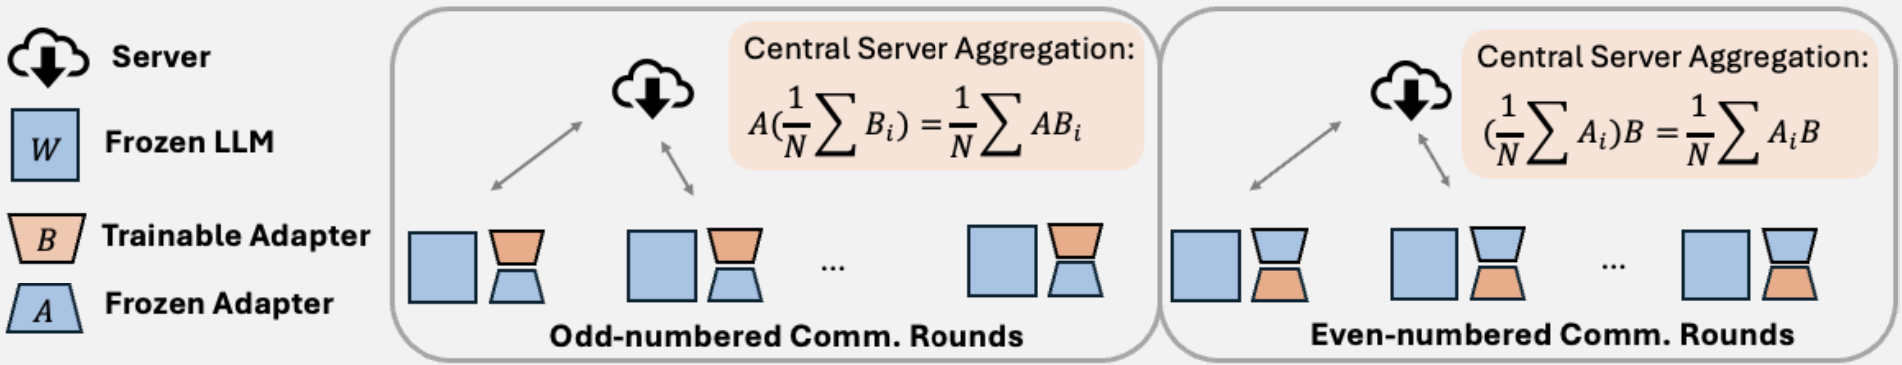
\includegraphics[width=0.75\textwidth]{figures/rolora_framework.png}
    \caption[Robust Low-Rank Adaptation (RoLoRA) alternating optimization scheme.]{Robust Low-Rank Adaptation (RoLoRA) alternating optimization scheme. In each round, one low-rank matrix is frozen globally while the other is trained and aggregated linearly. \emph{Note: The schematic reproduced from Chen et al.~\cite{chen2025robust} uses row-vector notation ($AB$); under our standard column-vector convention ($BA$), odd rounds aggregate $(\frac{1}{N}\sum B_i)A$ and even rounds aggregate $B(\frac{1}{N}\sum A_i)$.}}
    \label{fig:rolora_framework}
\end{figure}

\noindent \emph{Note on notation:} While Chen et al. \cite{chen2025robust} designate their low-rank product as $AB$ by naming the up-projection $A$ and down-projection $B$, we maintain the standard LoRA convention $\Delta W = \frac{\alpha}{r} BA$ \cite{hu2022lora} throughout this thesis to preserve mathematical consistency with common PEFT architectures and the formal framework developed in Chapter~\ref{chap:methodology}.

In odd-numbered communication rounds ($2t+1$), the down-projection matrix $A^t$ is globally frozen and shared across all clients $i$, while only the up-projection matrix $B$ is trained locally. The server then aggregates these updates:
\begin{equation}
    B^{t+1} = \frac{1}{N} \sum_{i=1}^{N} B^{t+1}_i
    \label{eq:rolora_B_agg}
\end{equation}
Because $A^t$ is identical across all clients, the aggregation is strictly linear, introducing no spatial interference:
\begin{equation}
    \frac{1}{N} \sum_{i=1}^{N} (B^{t+1}_i A^t) = \left( \frac{1}{N} \sum_{i=1}^{N} B^{t+1}_i \right) A^t = B^{t+1} A^t
    \label{eq:rolora_B_proof}
\end{equation}

In even-numbered communication rounds ($2t+2$), the aggregated up-projection matrix $B^{t+1}$ is frozen, while the clients update the down-projection matrix $A$ locally. The server aggregates these updates:
\begin{equation}
    A^{t+1} = \frac{1}{N} \sum_{i=1}^{N} A^{t+1}_i
    \label{eq:rolora_A_agg}
\end{equation}
Since $B^{t+1}$ is now identical across all clients, linearity is preserved:
\begin{equation}
    \frac{1}{N} \sum_{i=1}^{N} (B^{t+1} A^{t+1}_i) = B^{t+1} \left( \frac{1}{N} \sum_{i=1}^{N} A^{t+1}_i \right) = B^{t+1} A^{t+1}
    \label{eq:rolora_A_proof}
\end{equation}
This alternating optimization enables full parameter space exploration while maintaining zero-interference linear aggregations throughout the federated training process.

\section{Federated Dynamic Averaging}
\label{sec:fda}
Having resolved the spatial communication bottleneck through RoLoRA's linearized aggregation, we now address the temporal dimension: controlling the synchronization frequency based on actual training dynamics rather than a fixed schedule.

Federated Dynamic Averaging (FDA) and its optimization variant FDA-Opt \cite{theologitis2025fda} were developed to optimize the training schedule dynamically. FDA is rooted in the principles of Geometric Monitoring \cite{sharfman2006geometric}, a framework originally developed for threshold function monitoring over distributed data streams.

\subsection{Geometric Monitoring Foundations}
The core insight of geometric monitoring is that a global condition over distributed data can be decomposed into local conditions that each node monitors independently. Consider $N$ distributed nodes, each holding a local state vector $v_i(t)$ that evolves over time. The global state is the average $\bar{v}(t) = \frac{1}{N}\sum_{i=1}^{N} v_i(t)$. The monitoring objective is to detect when a threshold function $f(\bar{v}(t))$ crosses a predefined boundary, without requiring continuous global synchronization.

Geometric monitoring achieves this through the concept of \emph{safe zones}. Each node $i$ defines a bounding region around a reference point $e_i$ (typically the last synchronized global estimate). As long as the local drift vector $\delta_i(t) = v_i(t) - e_i$ remains within its safe zone, the global condition is guaranteed to hold by a convexity argument: if all local states lie within a convex safe zone centered around the global reference, their average must also lie within that zone. Crucially, this means that \emph{no communication is necessary} as long as every node's local constraint is satisfied. A synchronization round is triggered only when at least one node's drift exits its safe zone, indicating that the global condition may have been violated.

FDA adapts this distributed monitoring framework to the federated learning setting. The ``state vectors'' become local model parameter updates, the ``threshold function'' becomes model variance (measuring client drift divergence), and the ``safe zone'' is defined by a variance budget $\theta$. When local parameter drift across clients causes the variance to exceed $\theta$, synchronization is triggered. This reformulation transforms the rigid, schedule-based synchronization of standard FL into an event-driven protocol that communicates only when training dynamics demand it.

For a sampled subset of clients $S_t$ at communication round $t$, let $\Delta_{t,i}^{(k)} = w_{t,i}^{(k)} - w_{t,0}$ denote the local update of client $k$ at step $i$ relative to the initial global model $w_{t,0}$. The average update (pseudo-gradient) across all clients is defined as:
\begin{equation}
    g_{t,i} = \frac{1}{|S_t|} \sum_{k \in S_t} \Delta_{t,i}^{(k)}
    \label{eq:fda_pseudo}
\end{equation}
The model variance quantifies the dispersion of local client updates in the parameter space and is defined as:
\begin{equation}
    \text{Var}(W_{t,i}) = \frac{1}{|S_t|} \sum_{k \in S_t} \left\| \Delta_{t,i}^{(k)} \right\|_2^2 - \left\| g_{t,i} \right\|_2^2
    \label{eq:fda_variance}
\end{equation}
Here, the first term measures the average local training progress across clients, while the second term captures the magnitude of the aggregated global step. Consequently, a low model variance value signifies either negligible local gradient progress or, more favorably, highly aligned local updates across participating clients where local optimization trajectories coincide. Conversely, a high variance reading manifests when clients achieve substantial local parameter movement along divergent optimization vectors towards conflicting local minima, signaling the onset of severe client drift.


During local training, clients track model variance. Computing this exact variance requires full-dimensional vector operations, which can be computationally expensive and communication-heavy to track continuously in a distributed setting. To address this, the original FDA protocol utilizes the Alon-Matias-Szegedy (AMS) sketch \cite{alon1996space}, a randomized algorithm that efficiently approximates the $L_2$ norm (and thus the variance) using minimal memory and sub-linear space. While full-parameter models require randomized sketching to approximate variance in sub-linear memory, we show in Chapter~\ref{chap:methodology} that restricting geometric monitoring to compact low-rank coordinate tensors allows exact variance evaluation with negligible computational and memory overhead, rendering probabilistic sketching unnecessary in federated LoRA regimes.

Synchronization is triggered immediately if the variance exceeds a dynamic threshold: $\text{Var}(W_{t,i}) > \theta_t$. Because the variance magnitude evolves by orders of magnitude from early to late training stages, FDA-Opt dynamically scales this threshold across rounds using a linear prediction based on the previous round's termination step $s_t$:
\begin{equation}
    \theta_{t+1} = \text{var}_t \cdot \frac{\tau}{2 s_t}
    \label{eq:fda_threshold}
\end{equation}
where $\text{var}_t$ is the actual variance at termination in round $t$, $s_t$ is the termination step, and $\tau$ is the target training duration. This linear threshold prediction assumes that standard training variance typically grows linearly and monotonically during a round. Furthermore, to eliminate the synchronization overhead of checking variance at every training step, queries are restricted to a sparse subset of steps (typically once per epoch), mitigating the communication bottleneck of distributed geometric checks.

While RoLoRA resolves the spatial aggregation inconsistency and FDA addresses the temporal communication cadence, combining the two paradigms requires careful algorithmic formulation. In particular, low-rank parameter trajectories exhibit heightened variance volatility, and alternating optimization demands decoupled threshold management. To address these challenges, Chapter~\ref{chap:methodology} formalizes \textbf{FDA-RoLoRA} to combine dynamic averaging with alternating low-rank adaptation, explaining how it internally deploys a dual-track threshold mechanism to track subspace divergence independently. The concrete execution loops of both baseline protocols are formally summarized in Section~\ref{sec:foundational_protocols} before introducing our synthesized methodology.
